% Template LaTeX para impressão a um lado para relatórios, trabalhos académicos ou teses da Coimbra Business School / ISCAC
% Adaptado por Tiago Gualdrapa Soares (https://github.com/gualdrapa/CBS_LaTex_OneSided_Report_PT)
% Baseado originalmente no Template de Sven Hinz (https://github.com/SvenHinz) para relatórios e teses na Faculdade de Biomédica da FH Aachen


% Documento optimizado para impressão a um lado.
						 
% It is possible to change the layout to a twosided document by changing the class to \documentclass[twoside,openright,12pt,a4paper]{scrreprt} and adjusting the geometry \usepackage[left=2.5cm,right=1.5cm,top=2.5cm,bottom=2.5cm]{geometry} 
% But there might be problems with footer and header.
% ihead needs to be changed from \ihead[\sffamily \bfseries \upshape \headmark]{\sffamily \bfseries \upshape \headmark} to \ihead[]{}

% para resolver o erro scrpage2
\RequirePackage{scrlfile}
\ReplacePackage{scrpage2}{scrlayer-scrpage}


\documentclass[oneside,openright,12pt,a4paper]{scrreprt}

% Paket für Umlaute (für Deutsch):
\usepackage[utf8]{inputenc}       % Cross Platform
\usepackage{hyperref}   %links in TOC
\hypersetup{
    colorlinks=false, %set true if you want colored links of references and crossreferences
    linktoc=all,     %set to all if you want both sections and subsections linked
}

\usepackage[german,english,portuguese]{babel}       % language: germena nad english, english is main language, german is used in the german abstract and the acknowledgements 
\usepackage[ddmmyyyy]{datetime} 
\renewcommand{\dateseparator}{.} 
\usepackage{amsmath}
\usepackage{amsfonts}
\usepackage{amssymb}
\usepackage{makeidx}
\usepackage{graphicx}
\usepackage{epstopdf}
\usepackage{kpfonts}
\usepackage{blindtext}
\usepackage[left=2.0cm,right=2.0cm,top=2.5cm,bottom=2.5cm]{geometry} 

\newcommand\tab[1][1cm]{\hspace*{#1}}

\author{Tiago Gualdrapa Soares} % --> insert your name

\usepackage[automark,plainheadsepline,headsepline]{scrpage2}
\usepackage{color}
\usepackage{setspace}
\usepackage[numbers,sort&compress,square]{natbib} %this bibstyle uses numbers, which are sorted (increasing) and summarized eg. 104,105,106 --> 104-106 
\usepackage{longtable} 
\usepackage{listings}
\usepackage{rotating}
\usepackage{pdfpages}
\usepackage{caption}
\usepackage{subcaption}
\parindent 0pt
\usepackage{booktabs}
\usepackage[export]{adjustbox}
\usepackage{svg}

% to do inline lists
\usepackage[inline]{enumitem}


% fonts
\usepackage{helvet}
\renewcommand{\familydefault}{\sfdefault}
\setkomafont{chapter}{\sffamily \large}
\setkomafont{section}{\sffamily \normalsize}
\setkomafont{subsection}{\sffamily \normalsize}
\setkomafont{subsubsection}{\sffamily \normalsize}
\addtokomafont{caption}{\sffamily \small \itshape}
\usepackage{courier}
\usepackage{textgreek}
\usepackage{gensymb}
\setlength{\parindent}{0cm} %change indent of new paragraphs (if 0cm --> no indent)

% gap between header and headlines
\renewcommand*{\chapterheadstartvskip}{\vspace*{-0.75\baselineskip}}

% header and footer
\pagestyle{scrheadings}
\ohead[\sffamily \bfseries \upshape \headmark]{\sffamily \bfseries \upshape \headmark}
\chead[]{}
\ihead[]{}
\ofoot[\sffamily \pagemark]{\sffamily \pagemark}
\ifoot[]{}
\cfoot[]{}
\automark[]{chapter}
\renewcommand*{\chapterheadendvskip}{\vspace*{1\baselineskip}}

% formulas
\usepackage{fleqn} % left
\setlength{\mathindent}{1.5cm} % indent

% package for SI-units
\usepackage{siunitx}

%numbering of tables and figures (if you delete these, the figures and tables will be numbered according the chapter numbers)
\usepackage{chngcntr}
\counterwithout{figure}{chapter}
\counterwithout{table}{chapter}

% tables
\usepackage{multirow} % multilines in one column
\renewcommand{\arraystretch}{1.5} % increase (or decrease) line spacing in tables
\setlength{\doublerulesep}{0.2mm} % spacing between doubled lines 
\usepackage{tabu}
\newcolumntype{C}[1]{>{\centering\let\newline\\\arraybackslash\hspace{0pt}}m{#1}}
\newcolumntype{P}[1]{>{\raggedright\arraybackslash}p{#1}}


% command line
\lstdefinestyle{BashInputStyle}{
  language=bash,
  basicstyle=\small\ttfamily,
   frame=tb,
  columns=fullflexible,
  linewidth=0.9\linewidth,
  xleftmargin=0.1\linewidth
}

% Renaming "table of contents" in "Contents"
\renewcaptionname{english}{\contentsname}{\textbf{Contents}}

% Renaming "Sources" in "References"
\renewcaptionname{english}{\bibname}{\textbf{References}} 

\usepackage[
  tocindentmanual,
  tocflat,
  tocbreaksstrict,
  toctextentriesleft,
]{tocstyle}

\usepackage[]{acronym}

\usepackage{epigraph} %citacao no inicio do trabalho
\usepackage{footnote} %para usar notas de rodape
\usepackage[symbol]{footmisc}
\renewcommand{\thefootnote}{\fnsymbol{footnote}}
%\footnote[number]{text}
% 1 asterisk *
%2 dagger †
% 3 double dagger ‡
% 4 section symbol §
% 5 paragraph ¶
% 6 parallel lines ‖
% 7 two asterisks **
% 8 two daggers ††
% 9 two double daggers ‡‡



\makesavenoteenv{tabular}
%\usepackage{bidi} %precisa do xelatex
%\usepackage{bidiftnxtra}
\usepackage{tablefootnote}


\usepackage{eurosym}

%start of the document

\begin{document}
    \setstretch{1.5}
    \addtocontents{toc}{\linespread{1}}
    
    % Here the individual chapters are included in the main document by '\include{....}' . The files are in the folder 'doc'
        \begin{titlepage}

	\thispagestyle{empty}
	\newgeometry{left=0cm, right=0cm, top=0.6cm, bottom=0cm, includefoot}
	
	% FH Logo
	\begin{flushleft} ~\\ \vspace{-12mm} \hspace{12mm} 
		
\includegraphics[width=9.0cm]{./pic/CBS_Logo.jpg}
	\end{flushleft}

	\vspace{-2.5cm}
	
	% header
	\vspace{2.0cm}
	\centering \bfseries \Large Coimbra Business School \\
	\centering \bfseries \large Escola de Negócios de Coimbra
	\vspace{2.5cm}
	\normalsize 

	% title
	\centering \begin{minipage}[t]{17cm}
		\centering \bfseries \large Titulo \\
		 Continuação do Titulo ou Subtítulo
		\medskip
	\end{minipage}

	\vspace{3.5cm}

	\begin{minipage}[t]{10cm}
	\centering Pós-graduação em\\
	 Avaliação e Gestão da Actividade Imobiliária \\
		\centering \large Nome do autor %\\ Nome do co-autor
	\end{minipage}
		
    \vspace{3cm}
    \normalsize Unidade Curricular
    %\normalsize ISCAC - Instituto Superior de \\
   %Contabilidade e Administração de Coimbra \\
   %\centering \bfseries \small Instituto Politécnico de Coimbra
	%\vspace{2.1cm}
	
	%if needed add another logo of the institute or company
	%\begin{flushleft}
	%\centering \hspace{-2.5cm}
	%\begin{minipage}[t]{5cm}
	%		\includegraphics[width=1.7cm,rotate=-90]{./pic/xxx.jpg}
	%\end{minipage}
	%\end{flushleft}

    \vspace{3.5cm}
	\centering %\hspace{8cm}
	\begin{minipage}[b]{7cm}
			\centering
			Coimbra, 25 de Julho de 2020\\
	\end{minipage}
	
	\restoregeometry
	
\end{titlepage}

%add an empty page
% comentar as tres linhas seguinte para remover a pagina em branco depois da pagina de titulo (capa)
\newpage
    \thispagestyle{empty}
    \mbox{}
    \pagenumbering{gobble} %no page numbering
    \clearpage

\markboth{\textbf{Declaração}}{\textbf{Declaração}}
\mbox{}
\vspace{1.5cm}\\
\noindent 

Este trabalho foi realizado e escrito pelo autor. Nenhumas outras fontes para além das mencionadas foram usadas.\\
O autor declara a não existência de conflito de interesses ou outros interesses a declarar.

\vspace{1cm}
Nome do autor \tab[1.5cm] \rule{40mm}{0.2mm}\\
\tab[75mm] Assinatura

\vspace{25mm}
Este trabalho foi enviado por email para:

	\begin{minipage}[t]{13cm}
		\centering 
		\begin{tabular}{p{8cm}l}
			Professor Nome do professor \\
			email do professor
%			1. Pr\"{u}fer: & ~Prof. Dr. XXX\\
%			2. Pr\"{u}fer: & ~Dr. XYZ\\
	
		%\renewcommand{\arraystretch}{0.8}
		%	\begin{tabular}[c]{@{}l@{}}2. Pr\"{u}ferin \\ und Betreuerin:\end{tabular}
		%	&
		%\renewcommand{\arraystretch}{0.8}
		%	\begin{tabular}[c]{@{}l@{}} \\ YYY, M.Sc.\end{tabular}\\
		%\renewcommand{\arraystretch}{2.0}
%	        Betreuer: & ZZZ\\
			
		\end{tabular}
	\end{minipage}
	
	
	
	\vspace{45mm}
Contactos:

	\begin{minipage}[t]{13cm}
		\centering 
		\begin{tabular}{p{6cm}l}
			Nome do autor\\
			Email: & Email do autor\\
			Web: & Webpage do autor, Researchgate, etc.\\
%			1. Pr\"{u}fer: & ~Prof. Dr. XXX\\
%			2. Pr\"{u}fer: & ~Dr. XYZ\\
	
		%\renewcommand{\arraystretch}{0.8}
		%	\begin{tabular}[c]{@{}l@{}}2. Pr\"{u}ferin \\ und Betreuerin:\end{tabular}
		%	&
		%\renewcommand{\arraystretch}{0.8}
		%	\begin{tabular}[c]{@{}l@{}} \\ YYY, M.Sc.\end{tabular}\\
		%\renewcommand{\arraystretch}{2.0}
%	        Betreuer: & ZZZ\\
			
		\end{tabular}
	\end{minipage}

	\vspace{1.5cm}
\newpage
    \thispagestyle{empty}
    \mbox{}
    \setcounter{page}{1} %counter for page numbering is set to 1
    \pagenumbering{Roman} % page numbering is done with capital roman signs (I, II, III...)
    \clearpage
\thispagestyle{empty}

%\markboth{\textbf{Declaração}}{\textbf{Declaração}}
%\mbox{}
%\vspace{1.5cm}\\
%\noindent 

%\vspace{40mm}
%\vspace*{\fill}
\vspace*{30mm}
\setlength\epigraphwidth{.55\textwidth}
%\setlength\epigraphrule{0pt}

\epigraph{``All our dreams can come true, if we have the courage to pursue them.''\\ \hfill \textit{Walt Disney}} 




\newpage
    \thispagestyle{empty}
    \mbox{}
    %\clearpage

%\markboth{\textbf{Abstract}}{\textbf{Abstract}}\label{abstract}
%This is the english abstract 

%\clearpage

%\markboth{\textbf{Zusammenfassung}}{\textbf{Zusammenfassung}}\label{Zusammenfassung}
%Hier kommt die deutsche Zusammenfassung

\clearpage

\markboth{\textbf{Resumo}}{\textbf{Resumo}}\label{Resumo}
\begin{center}
\textbf{Titulo}
\\
\center{\textbf{\large{RESUMO}}}
\end{center}

\vspace{7mm}



\textbf{Objectivo:} Lorem ipsum dolor sit amet, consectetur adipiscing elit, sed do eiusmod tempor incididunt ut labore et dolore magna aliqua. Ut enim ad minim veniam, quis nostrud exercitation ullamco laboris nisi ut aliquip ex ea commodo consequat. Duis aute irure dolor in reprehenderit in voluptate velit esse cillum dolore eu fugiat nulla pariatur. Excepteur sint occaecat cupidatat non proident, sunt in culpa qui officia deserunt mollit anim id est laborum. 

\textbf{Design/Metodologia/Abordagem:} Lorem ipsum dolor sit amet, consectetur adipiscing elit, sed do eiusmod tempor incididunt ut labore et dolore magna aliqua. Ut enim ad minim veniam, quis nostrud exercitation ullamco laboris nisi ut aliquip ex ea commodo consequat.

\textbf{Descobertas:} Lorem ipsum dolor sit amet, consectetur adipiscing elit, sed do eiusmod tempor incididunt ut labore et dolore magna aliqua. Ut enim ad minim veniam, quis nostrud exercitation ullamco laboris nisi ut aliquip ex ea commodo consequat. Duis aute irure dolor in reprehenderit in voluptate velit esse cillum dolore eu fugiat nulla pariatur. Excepteur sint occaecat cupidatat non proident, sunt in culpa qui officia deserunt mollit anim id est laborum.

\textbf{Limitações da investigação/Implicações:} Lorem ipsum dolor sit amet, consectetur adipiscing elit, sed do eiusmod tempor incididunt ut labore et dolore magna aliqua. Ut enim ad minim veniam, quis nostrud exercitation ullamco laboris nisi ut aliquip ex ea commodo consequat.

\textbf{Implicações práticas:} Lorem ipsum dolor sit amet, consectetur adipiscing elit, sed do eiusmod tempor incididunt ut labore et dolore magna aliqua. Ut enim ad minim veniam, quis nostrud exercitation ullamco laboris nisi ut aliquip ex ea commodo consequat. Duis aute irure dolor in reprehenderit in voluptate velit esse cillum dolore eu fugiat nulla pariatur. Excepteur sint occaecat cupidatat non proident, sunt in culpa qui officia deserunt mollit anim id est laborum.


\textbf{Originalidade/Valor:} Lorem ipsum dolor sit amet, consectetur adipiscing elit, sed do eiusmod tempor incididunt ut labore et dolore magna aliqua. Ut enim ad minim veniam, quis nostrud exercitation ullamco laboris nisi ut aliquip ex ea commodo consequat.

\vspace*{\fill}
\textbf{Palavras-chave:} palavra1, palavra2, palavra3, palavra4, palavra5, palavra6.

\newpage
    \thispagestyle{empty}
    \mbox{}
    %\clearpage

%\markboth{\textbf{Abstract}}{\textbf{Abstract}}\label{abstract}
%This is the english abstract 

%\clearpage

%\markboth{\textbf{Zusammenfassung}}{\textbf{Zusammenfassung}}\label{Zusammenfassung}
%Hier kommt die deutsche Zusammenfassung

\clearpage

\markboth{\textbf{Resumo}}{\textbf{Abstract}}\label{Abstract}
\begin{center}
\textbf{Title}
\\
\center{\textbf{\large{ABSTRACT}}}
\end{center}

\vspace{7mm}

\textbf{Purpose:} Lorem ipsum dolor sit amet, consectetur adipiscing elit, sed do eiusmod tempor incididunt ut labore et dolore magna aliqua. Ut enim ad minim veniam, quis nostrud exercitation ullamco laboris nisi ut aliquip ex ea commodo consequat. Duis aute irure dolor in reprehenderit in voluptate velit esse cillum dolore eu fugiat nulla pariatur. Excepteur sint occaecat cupidatat non proident, sunt in culpa qui officia deserunt mollit anim id est laborum. 

\textbf{Design/Methodology/Approach:} Lorem ipsum dolor sit amet, consectetur adipiscing elit, sed do eiusmod tempor incididunt ut labore et dolore magna aliqua. Ut enim ad minim veniam, quis nostrud exercitation ullamco laboris nisi ut aliquip ex ea commodo consequat.

\textbf{Findings:} Lorem ipsum dolor sit amet, consectetur adipiscing elit, sed do eiusmod tempor incididunt ut labore et dolore magna aliqua. Ut enim ad minim veniam, quis nostrud exercitation ullamco laboris nisi ut aliquip ex ea commodo consequat. Duis aute irure dolor in reprehenderit in voluptate velit esse cillum dolore eu fugiat nulla pariatur. Excepteur sint occaecat cupidatat non proident, sunt in culpa qui officia deserunt mollit anim id est laborum.

\textbf{Research limitations/Implications:} Lorem ipsum dolor sit amet, consectetur adipiscing elit, sed do eiusmod tempor incididunt ut labore et dolore magna aliqua. Ut enim ad minim veniam, quis nostrud exercitation ullamco laboris nisi ut aliquip ex ea commodo consequat.

\textbf{Practical implications:} Lorem ipsum dolor sit amet, consectetur adipiscing elit, sed do eiusmod tempor incididunt ut labore et dolore magna aliqua. Ut enim ad minim veniam, quis nostrud exercitation ullamco laboris nisi ut aliquip ex ea commodo consequat. Duis aute irure dolor in reprehenderit in voluptate velit esse cillum dolore eu fugiat nulla pariatur. Excepteur sint occaecat cupidatat non proident, sunt in culpa qui officia deserunt mollit anim id est laborum.


\textbf{Originality/Value:} Lorem ipsum dolor sit amet, consectetur adipiscing elit, sed do eiusmod tempor incididunt ut labore et dolore magna aliqua. Ut enim ad minim veniam, quis nostrud exercitation ullamco laboris nisi ut aliquip ex ea commodo consequat.


\vspace*{\fill}
\textbf{Keywords:} keyword1, keyword2, keyword3, keyword4, keyword5, keyword6.

\newpage
    \thispagestyle{empty}
    \mbox{}
    
    % Table of contents is generated:
    \makeatletter
    \renewcommand*{\@dotsep}{1} % set gap between dots
    \makeatother
    \tableofcontents
   
    % First chapter starts on uneven number 
    \cleardoublepage
    \setstretch{1.25}
    \pagenumbering{arabic} %page numbering is done with arabic numbers
    % chapters which are not used can be commented out
    % additional chapters require a new file in folder 'doc'
    \clearpage

%\onehalfspacing
\chapter{\textbf{Introdução}}\label{intro}



\section{Background}

\blindtext

\section{Justificação e objectivos do trabalho}

\blindtext

\section{Metodologia de investigação}

\blindtext

\section{Limitações}

\blindtext

\section{Organização do trabalho}

\blindtext



%\section{Objectivos e motivação}
%\blindtext






%\section{Problema e objectivo}\label{objectives}



\addtocontents{toc}{\vspace{0.8cm}}
 % Introduction 
    \chapter{\textbf{Estado da arte e base teórica}}

\section{Primeira secção}
%blindtext is used to generate a random text to show how text looks in the pdf
\Blindtext

%example for a figure, figures should be saved in the folder 'fig'
\begin{figure}[ht]
	\centering

		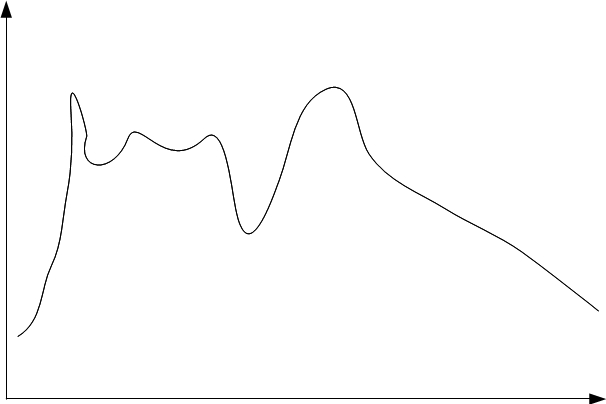
\includegraphics[width=0.8\textwidth]{pic/example.jpg}

	\caption[First example.]{First example to describe how short and long caption work for figures. Everything written in the square brackets will be listed in the list of figures, everything written in the curly brackets will be shown directly underneath the figure.}

	\label{fig:firstexample}
\end{figure}




%example for a crossreference (here: figure)
Here I will reference the first figure (see figure \ref{fig:firstexample}). Also, in \ref{res:subfigure} a figure with multiple subfigures is shown.

\noindent %no indent is generated in the new paragraph
The we can make a list of different things:

%example for a list without numbers
\begin{itemize} 
\item First item on the list
\item Second item on the list 
\item Third item on the list 
\end{itemize}


\section{Segunda secção}

Outro tipo de lista:

\begin{itemize}[noitemsep]
%\setlength\itemsep{1em}
\item[--] \textbf{Item 1:} Descrição do primeiro item;
\item[--] \textbf{Item 2:} Descrição do segundo item;
\item[--] \textbf{Item 4:} Descrição do terceiro item;
\item[--] \textbf{Item 5:} Descrição do quarto item;
\end{itemize}


\addtocontents{toc}{\vspace{0.8cm}} % -> add space in TOC  % State of the art
    \clearpage

\chapter{\textbf{Métodos}}\label{methods}

\section{Inicio de um capítulo}\label{met:chapters}
In the two-sided layout a new chapter always begins on a right side. Therefore, empty pages will be generated automatically at the end of the previous chapter if necessary. The one-sided layout does not do this. If you want an additional empty page, you have to insert it manually.

\section{Tabelas grandes}\label{met:table}
Tables are a bit complex to generate in latex, a big help are table generators like: \url{https://www.tablesgenerator.com/} . Small tables fit within the text flow. \\
\begin{table} [ht]
    \begin{center}
    %\centering
         \caption[Small table]{Material needed for gels
         }
\begin{tabular}{|l|C{3cm}|C{3cm}|}
\hline
material (conc.) & volume per gel & conc. in gel\\ \hline
Chemical 1 (40~mg/mL)             & 15~\textmu L     & 3.00~ \textmu g/mL\\ \hline
TBS                             & 15~\textmu L     & ---\\ \hline
Chemical 2         & 15~\textmu L     & 3.75~\textmu g/mL\\ \hline
Chemical 3   & 27.5~\textmu L   & 5.7x10$^5$ cells\\ \hline
Chemical 4  & 27.5~\textmu L   & 5.7x10$^5$ cells\\ \hline \hline 
Chemical 5      & 100~\textmu L    & 5.00 mg/mL \\ \hline

        \end{tabular}
 \label{tabfibrin}
    \end{center}
\end{table}
Bigger tables can be put on separate pages. \\


\begin{table} [p] %p makes to table to show up on a separate page. This is useful when the table is really big or two tables should be aligned underneath each other on a separate page.

    \begin{center}
    \caption[FACS analysis]{A lot of complex columns and rows
         }
\begin{tabular}{|l|l|l|l|l|l|l|l|l|l|l|}
\hline
\multicolumn{2}{|c|}{Tube 1}                                 &                       & \multicolumn{2}{c|}{Tube 2}                                 &  & \multicolumn{2}{c|}{Tube 3}                                 & \multicolumn{1}{c|}{} & \multicolumn{2}{c|}{Tube 4}                                 \\ \cline{1-2} \cline{4-5} \cline{7-8} \cline{10-11} 
\multicolumn{1}{|c|}{Antibody} & \multicolumn{1}{c|}{Volume} & \multicolumn{1}{c|}{} & \multicolumn{1}{c|}{Antibody} & \multicolumn{1}{c|}{Volume} &  & \multicolumn{1}{c|}{Antibody} & \multicolumn{1}{c|}{Volume} & \multicolumn{1}{c|}{} & \multicolumn{1}{c|}{Antibody} & \multicolumn{1}{c|}{Volume} \\ \cline{1-2} \cline{4-5} \cline{7-8} \cline{10-11} 
AB1   & 20~\textmu L   &    & AB2    & 20~\textmu L  &  & AB3    & 20~\textmu L    &     & AB4      &20~\textmu L       \\ 
\cline{1-2} \cline{4-5} \cline{7-8} \cline{10-11}  
APC   & MSC-   &  & FITC  & MSC- &  & PE   & MSC-  & & PE   & MSC-    \\
\cline{1-2} \cline{4-5} \cline{7-8} \cline{10-11} 
\multicolumn{1}{|c|}{Antibody} & \multicolumn{1}{c|}{Volume} & \multicolumn{1}{c|}{} & \multicolumn{1}{c|}{Antibody} & \multicolumn{1}{c|}{Volume} &  & \multicolumn{1}{c|}{Antibody} & \multicolumn{1}{c|}{Volume} & \multicolumn{1}{c|}{} & \multicolumn{1}{c|}{Antibody} & \multicolumn{1}{c|}{Volume}\\ 
\cline{1-2} \cline{4-5} \cline{7-8} \cline{10-11} 
AB5  & 2~\textmu L   &   & AB6   & 5~\textmu L  &  & AB7   & 5~\textmu L         &    & AB8    & 5~\textmu L    \\ 
\cline{1-2} \cline{4-5} \cline{7-8} \cline{10-11} 
FITC  & MSC+  &   & APC  & MSC+   &  & \scriptsize{PerCP-Cy5.5}  & MSC+  &  & \scriptsize{PerCP-Cy5.5}  & MSC-       \\ 
\hline
\end{tabular}
 \label{tabfacsmsc}
    \end{center}
\end{table}

\begin{table} [p]
    \begin{center}
    %\centering
         \caption[Another list of antibodies]{Some more antibodies for FACS analysis
         }
\begin{tabular}{|l|l|l|l|l|l|l|l|l|l|l|}
\hline
\multicolumn{2}{|c|}{Tube 1}                                 &                       & \multicolumn{2}{c|}{Tube 2}                                 &  & \multicolumn{2}{c|}{Tube 3}                                 & \multicolumn{1}{c|}{} & \multicolumn{2}{c|}{Tube 4}                                 \\ \cline{1-2} \cline{4-5} \cline{7-8} \cline{10-11} 
\multicolumn{1}{|c|}{Antibody} & \multicolumn{1}{c|}{Volume} & \multicolumn{1}{c|}{} & \multicolumn{1}{c|}{Antibody} & \multicolumn{1}{c|}{Volume} &  & \multicolumn{1}{c|}{Antibody} & \multicolumn{1}{c|}{Volume} & \multicolumn{1}{c|}{} & \multicolumn{1}{c|}{Antibody} & \multicolumn{1}{c|}{Volume} \\ \cline{1-2} \cline{4-5} \cline{7-8} \cline{10-11} 
AB1   & 20~\textmu L   &    & AB2    & 20~\textmu L  &  & AB3    & 5~\textmu L    &     & AB4      & 5~\textmu L       \\ 
\cline{1-2} \cline{4-5} \cline{7-8} \cline{10-11} 
FITC   & EC+   &  & FITC  & EC+ &  & FITC   & EC+  & & FITC   & EC-    \\
\cline{1-2} \cline{4-5} \cline{7-8} \cline{10-11} 
\multicolumn{1}{|c|}{Antibody} & \multicolumn{1}{c|}{Volume} & \multicolumn{1}{c|}{} & \multicolumn{1}{c|}{Antibody} & \multicolumn{1}{c|}{Volume} &  & \multicolumn{1}{c|}{Antibody} & \multicolumn{1}{c|}{Volume} & \multicolumn{1}{c|}{} & \multicolumn{1}{c|}{Antibody} & \multicolumn{1}{c|}{Volume}\\ 
\cline{1-2} \cline{4-5} \cline{7-8} \cline{10-11} 
AB5  & 20~\textmu L   &   & AB6   & 2~\textmu L  &  & AB7   & 20~\textmu L         &    & AB8    & 20~\textmu L    \\ 
\cline{1-2} \cline{4-5} \cline{7-8} \cline{10-11} 
APC  & EC-  &   & APC  & EC-   &  & APC  & EC+  &  & APC  & EC+       \\ 
\hline
\end{tabular}
 \label{tabfacsec}
    \end{center}
\end{table}

\blindtext
\section{Isto é uma secção}
\subsection{Isto é uma subsecção}
\subsubsection{Isto é uma subsubsecção que não aparece no índice}\label{subsub}
Here we have some random equations: 
\begin{equation}\label{Volume}
V = d^2\cdot \frac{\pi}{4}\cdot L
\end{equation}

\begin{equation}\label{Surface}
S = d^2 \cdot \frac{\pi}{4} + \pi \cdot d \cdot L \thickapprox \pi \cdot d \cdot L
\end{equation}

\begin{equation}\label{Volume1}
V = \frac{S^2}{\pi ^2 \cdot L^2} \cdot \frac{\pi}{4}\cdot L = \frac{S^2}{4\pi \cdot L}
\end{equation}
\begin{equation}\label{Length}
L = \frac{S^2}{4\pi \cdot V}
\end{equation}

\begin{equation}\label{stdv}
 s = \sqrt{\frac{\sum_{i=1}^n (x_i-\bar{x})^2}{(n-1)}}
\end{equation}

\newpage
\subsubsection{Outro tipo de tabelas}\label{outrotabelas}
\begin{table} [h!]
	\begin{center}
    %\centering
       
	\begin{tabular}{lcc}
	\toprule
	Indicador & Descrição & Unidade \\
	\midrule
	E1 & $\frac{\text{Custo Total de Manutenção}}{\text{Valor de substituição dos activos}}$ & $\times 100\%$ \\
	E2 & $\frac{\text{Custo Total de Manutenção}}{\text{Valor valor acrescentado + Custos Externos de Manutenção}}$ & $\times 100\%$ \\
	E3 & $\frac{\text{Custo Total de Manutenção}}{\text{Quantidade de \textit{Output}}}$ & \euro / Un. \\
	E5 & $\frac{\text{Custo Total de Manutenção + Custo de inoperação por manutenção}}{\text{Quantidade de \textit{Output}}}$ & \euro / Un. \\
	E7 & $\frac{\text{Valor médio do Stock de Materiais de Manutenção}}{\text{Valor de substituição dos activos}}$ & $\times 100\%$ \\
	E8 & $\frac{\text{Custo Total do pessoal interno de Manutenção}}{\text{Valor de substituição dos activos}}$ & $\times 100\%$ \\
	E9 & $\frac{\text{Custo Total do pessoal externo de Manutenção}}{\text{Valor de substituição dos activos}}$ & $\times 100\%$ \\
	E10 & $\frac{\text{Custo Total dos Serviços de Terceiros}}{\text{Valor de substituição dos activos}}$ & $\times 100\%$ \\
	E11 & $\frac{\text{Custo Total de Materiais de Manutenção}}{\text{Valor de substituição dos activos}}$ & $\times 100\%$ \\
	E12 & $\frac{\text{Custo Total de Materiais de Manutenção}}{\text{Valor médio do stock de Materiais de Manutenção}}$ & $\text{rotações / ano}$ \\
	E15 & $\frac{\text{Custo de Manutenção Correctiva}}{\text{Valor médio do stock de Materiais de Manutenção}}$ & $\times 100\%$ \\
	E16 & $\frac{\text{Custo de Manutenção Preventiva}}{\text{Valor médio do stock de Materiais de Manutenção}}$ & $\times 100\%$ \\
	E19 & $\frac{\text{Custo de Manutenção de Melhoria}}{\text{Valor médio do stock de Materiais de Manutenção}}$ & $\times 100\%$ \\

	\bottomrule

	\end{tabular}
    \caption[Lista (não extensiva) de indicadores-chave económicos]{Lista (não extensiva) de indicadores-chave económicos}              
	\label{tab:indicadore_economicos}
    \end{center}
\end{table}



\addtocontents{toc}{\vspace{0.8cm}} % Methods
    \clearpage

\chapter{\textbf{Resultados}}\label{results}
\section{Figura com subfiguras}\label{res:subfigure}
As in this case the figure with subfigures is quite big, it will appear in the next page. If they are smaller, they also fit within the text flow.\\
In the square brackets after 'begin figure' or 'begin subfigure, the command 'trim = l b r t' is cutting the figures on the left, bottom, right and top. Additionally, 'clip' is needed afterwards. 'rotate' can be used to rotate the figure. In the curly brackets the size of the figure can be adjusted either by using a defined width eg. 4~cm or by a percentage of the textwidth.
\begin{figure}[p]
    \centering % <-- added
\begin{subfigure}{0.75\textwidth}
  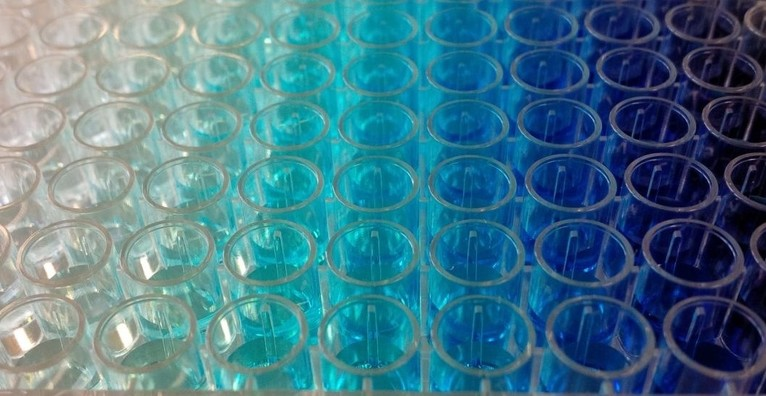
\includegraphics[trim = 30mm 15mm 0mm 20mm, clip,
  width=\linewidth]{pic/anyfigure.png}
  \caption{Caption for the first subfigure}
  \label{fig:1}
\end{subfigure}\hfil % <-- added
\begin{subfigure}{7 cm}
  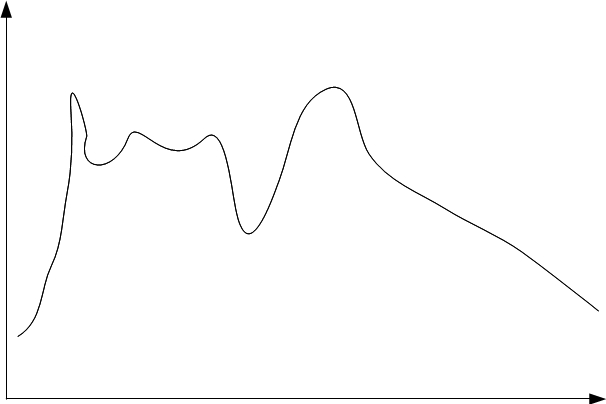
\includegraphics[trim = 30mm 15mm 0mm 20mm, clip, rotate=180, width=\linewidth]{pic/example.jpg}
  \caption{Caption for the second subfigure}
  \label{fig:2}
\end{subfigure}\hfil % <-- added

\medskip
\begin{subfigure}{0.75\textwidth}
  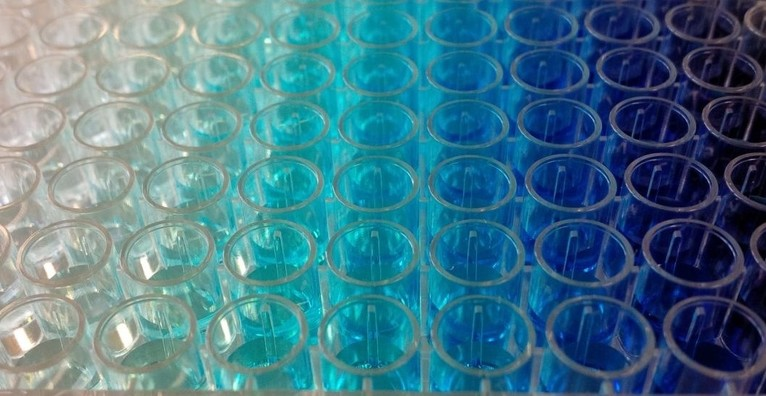
\includegraphics[trim = 30mm 15mm 0mm 20mm, clip, width=\linewidth]{pic/anyfigure.png}
  \caption{Caption for the third subfigure}
  \label{fig:3}
\end{subfigure}\hfil % <-- added

\caption[Figure with multiple subfigures]{3 subfigures can be combined in one figure. Each subfigure has a short caption and the figure itself has a caption underneath}
\label{fig:FACS-diff-comparison}
\end{figure}


\addtocontents{toc}{\vspace{0.8cm}} % Results
    \clearpage

\chapter{\textbf{Discussão}}\label{discussion}
\section{Referências bibliográficas no texto}
Here we want to discuss and will use some references from our bib file. \\
In the bib file all your references are collected. Best is to use google scholar (\url{https://scholar.google.com}), as you can directly copy the Latex code. To add a reference in your text, you cite it~\cite{Amini12}. By using the style unsrtdin and its extension, references are sorted automatically in the text~\cite{Amini12,Bajpai12}. Also, they are compressed if there are more than 3 references in 'a row'~\cite{Carpenter79,Davis11,Eurotransplant17,Falcone93}. The command 'nocite' is used to add a references to your List of References without mentioning in the text~\nocite{website:chick}.

\addtocontents{toc}{\vspace{0.8cm}} % Discussion
    \clearpage

\chapter{\textbf{Conclusão}}\label{conclusao}

Sed ut perspiciatis unde omnis iste natus error sit voluptatem accusantium doloremque laudantium, totam rem aperiam, eaque ipsa quae ab illo inventore veritatis et quasi architecto beatae vitae dicta sunt explicabo. Nemo enim ipsam voluptatem quia voluptas sit aspernatur aut odit aut fugit, sed quia consequuntur magni dolores eos qui ratione voluptatem sequi nesciunt. Neque porro quisquam est, qui dolorem ipsum quia dolor sit amet, consectetur, adipisci velit, sed quia non numquam eius modi tempora incidunt ut labore et dolore magnam aliquam quaerat voluptatem. Ut enim ad minima veniam, quis nostrum exercitationem ullam corporis suscipit laboriosam, nisi ut aliquid ex ea commodi consequatur? Quis autem vel eum iure reprehenderit qui in ea voluptate velit esse quam nihil molestiae consequatur, vel illum qui dolorem eum fugiat quo voluptas nulla pariatur?

\addtocontents{toc}{\vspace{0.8cm}} % Outlook
    %\include{./doc/107chapter7}
    %\include{./doc/108chapter8}

    % References
    \clearpage
    \bibliographystyle{unsrtdineng} % modified unsrtdin needs to be included as file in the main path (same level as the main document 000report.tex 
    \bibliography{./bib/quellen}
    \addcontentsline{toc}{chapter}{\textbf{Referências bibliográficas}}
     % add to TOC
    \clearpage
    
    %List of abbreviations
    \markright{\textbf{Lista de Abreviaturas}}
    \markleft{\textbf{Lista de Abreviaturas}}
    \clearpage
\chapter*{\textbf{Lista de Abreviaturas}}\label{abblist}
\addcontentsline{toc}{chapter}{\textbf{Lista de Abreviaturas}}
\begin{acronym}[YTM]
\setlength{\itemsep}{-\parsep}

\acro{ABM}[$ABM$]{\hspace{1.9cm}Antibiotic/Antimycotic}
\acro{AcLDL}[$AcLDL$]{\hspace{1.5cm} acetylated low density lipoprotein}
\acro{EGF}[$EGF$]{\hspace{2cm}Epidermal growth factor}
\acro{EGM-2}[$EGM\small{-2}$]{\hspace{1.38cm}Endothelial cell growth medium 2}
\acro{ELISA}[$ELISA$]{\hspace{1.62cm}Enzyme-linked immunosorbent assay}
\acro{FACS}[$FACS$]{\hspace{1.75cm}Fluorescence-activated cell sorting}
\acro{HE}[$HE$]{\hspace{2cm}Hematoxylin and eosin}
\acro{HEPES}[$HEPES$]{\hspace{1.42cm}4-(2-hydroxyethyl)-1-piperazineethanesulfonic acid}
\acro{RNA}[$RNA$]{\hspace{2cm}Ribonucleic acid}
\acro{RT}[$RT$]{\hspace{2cm}Room temperature}
\acro{vWf}[$vWf$]{\hspace{2cm}Von Willebrand factor}


\end{acronym}


    \clearpage
    
    %List of figures
    \markright{\textbf{Lista de Figura}}
    \markleft{\textbf{Lista de Figura}}
    \listoffigures 
    \addcontentsline{toc}{chapter}{\textbf{Lista de Figuras}}
    
    %List of tables
    \clearpage
    \markright{Lista de Tabelas}
    \markleft{Lista de Tabelas}
    \listoftables
    \addcontentsline{toc}{chapter}{\textbf{Lista de Tabelas}}
    \clearpage
    
    %acknowledgments 
    \clearpage
    \markright{Agradecimentos}
    \markleft{Agradecimentos}
    \clearpage
\chapter*{\textbf{Agradecimentos}}\label{Agradecimentos}

\addcontentsline{toc}{chapter}{\textbf{Agradecimentos}}
\selectlanguage{portuguese}
Se deseja escrever em alemão ou inglês aqui, o comando 'selectlanuage' chama a ortografia ou hifenização em alemão ou inglês.


%\addtocontents{toc}{\vspace{0.8cm}}

    
    
    %Appendix
    \clearpage

\chapter*{\textbf{Anexo}}\label{appendix}
\addcontentsline{toc}{chapter}{\textbf{Anexo}}
\markboth{\textbf{Anexo}}{\textbf{Anexo}}

\begin{figure}[htb]
	\centering
		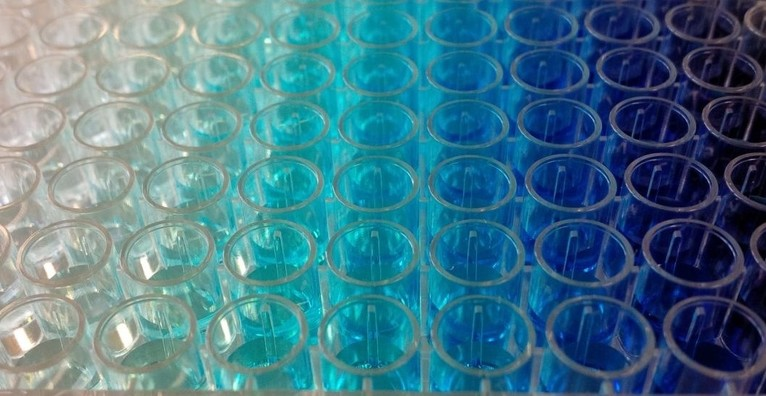
\includegraphics[width=0.9\textwidth]{pic/anyfigure.png}

	\caption[Cool picture]{Some cool photo taken in the lab.}

	\label{fig:anyfigure}
\end{figure}

\begin{figure}[htb]
	\centering

		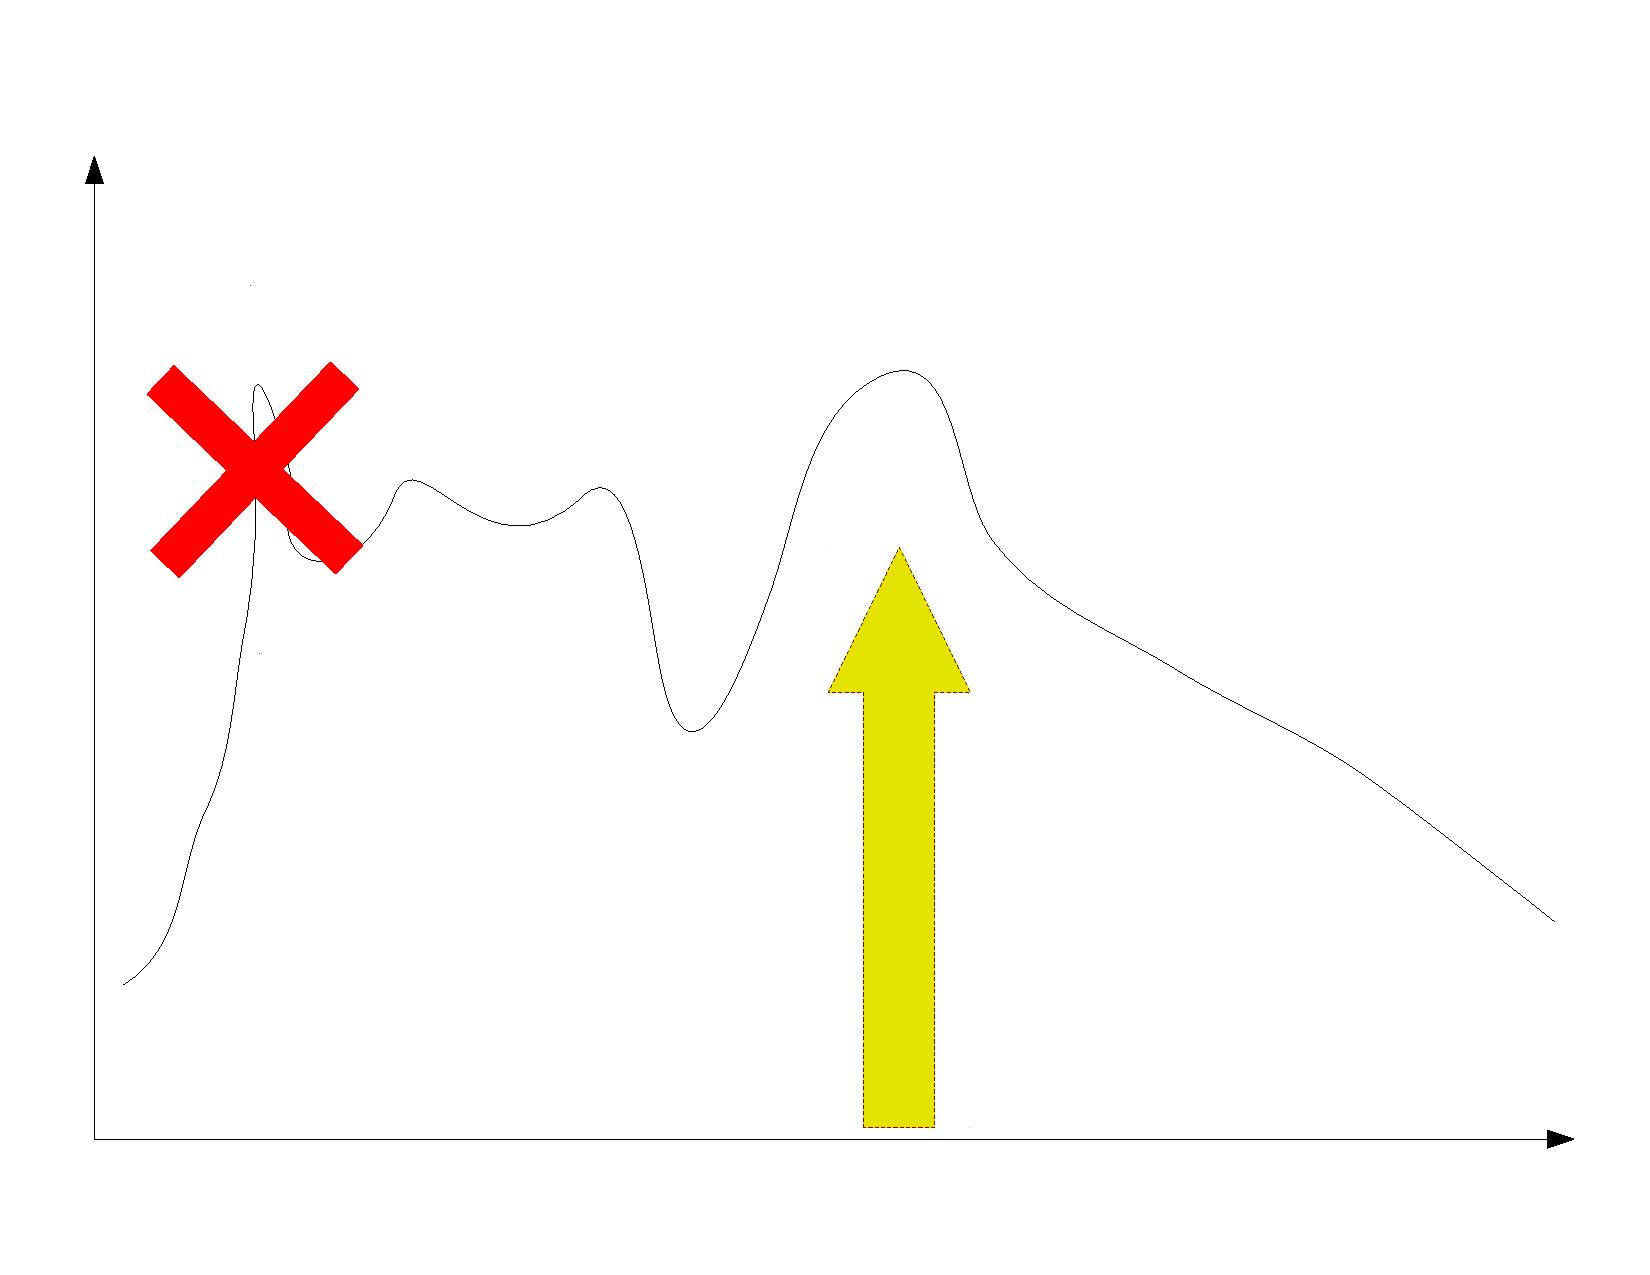
\includegraphics[trim = 15mm 70mm 20mm 20mm, clip, rotate=90,  width=0.5\textwidth]{pic/anypdf.pdf}

	\caption[Adding PDF as figure]{It is possible to add pdf files as figure, while keeping your header and footer from your document. Mostly useful in the appendix.}

	\label{fig:pdf}
\end{figure}

\end{document}
